\documentclass[11pt]{article}

%%
%% PACKAGES
%%

% Margins
\usepackage[margin=0.9in, top=0.8in, bottom=1.0in]{geometry}

% Fonts, typesetting, and math symbols
\usepackage[T1]{fontenc}
\usepackage{tgpagella} % Palatino-based font from TeX Gyre
\usepackage[scaled]{beramono} % Lovely monospace font
\usepackage{tgheros} % Helvetica-based font for headings
\usepackage{amsmath, amssymb}
\usepackage{mathtools}
\usepackage{mathdots}
\usepackage{microtype}
\usepackage{xspace}
\usepackage{xfrac}
\usepackage{calc}

% Plotting and drawing
\usepackage{tikz} % This automatically loads graphicx!
%\usetikzlibrary{calc} % For relative positions to defined coords
%\usepackage{pgfplots} % Scientific plotting tools
%\pgfplotsset{compat=1.7}

% Graphics
%\usepackage{graphicx}
%\usepackage[update,prepend]{epstopdf}
\usepackage{titlesec}
\usepackage{color}

% Table improvements
\usepackage{booktabs}

% Figure placement
%\usepackage{wrapfig}

% Code listings
\usepackage{listings}
\usepackage{matlab-prettifier}	% MATLAB code listings

% Tweaks for captions and enumerations
\usepackage[labelfont=bf]{caption}
%\captionsetup[wrapfigure]{margin=0.5cm}
\usepackage{enumitem}
\setlist[itemize]{itemsep=3pt,leftmargin=*,label=\textbullet}

% Fancy headers
\usepackage{fancyhdr}
\setlength{\headheight}{0pt}
\setlength{\footskip}{50pt}
\renewcommand{\headrulewidth}{0pt}
\renewcommand{\footrulewidth}{0pt}

%%
%% SETTINGS
%%

% Path to look for graphics
\graphicspath{{../images/}}

% Caption spacing
\setlength{\abovecaptionskip}{0pt}

% List spacing
\setlist{noitemsep}

% Table spacing
\renewcommand{\arraystretch}{1.3}

% Math operator font
% Note that cmr=roman and cmss=sans-serif.
\DeclareSymbolFont{sfoperators}{OT1}{cmr}{m}{n}
\DeclareSymbolFontAlphabet{\mathsf}{sfoperators}
\makeatletter
\def\operator@font{\mathgroup\symsfoperators}
\makeatother

%% No indent all paragraphs
%\setlength{\parindent}{0in}

% Figure and table references
\newcommand{\figref}[1]{Figure~\ref{#1}}
\newcommand{\tabref}[1]{Table~\ref{#1}}

% Special format section headings
\titleformat{\section}%
	{\color{blue}\large}% Text formatting
	{Part \arabic{section}}% Number
	{1em}% Space between number and text
	{}% Code before
	[\addvspace{-10pt}\rule{\textwidth}{0.4pt}]% Code after
\titleformat{\subsection}%
	{\color{blue}\normalsize\itshape}% Text formatting
	{Problem \arabic{section}.\arabic{subsection}}% Number
	{1em}% Space between number and text
	{}% Code before
	[\addvspace{-10pt}\rule{\widthof{Problem \arabic{section}.\arabic{subsection}}}{0.4pt}]% Code after
%\titleformat{\subsubsection}%
%	{\color{blue}}% Text formatting
%	{\arabic{subsubsection} $\rightarrow$}% Number
%	{1em}% Space between number and text
%	{}% Code before
%	[]% Code after

\definecolor{mygray}{rgb}{0.4, 0.4, 0.4}
\lstset{
style=Matlab-editor,
mlscaleinline=false,
basicstyle=\ttfamily\lst@ifdisplaystyle\scriptsize\fi,
frame=single,
rulecolor=\color{mygray},
numbers=left,
numbersep=10pt,
numberstyle=\footnotesize \ttfamily \color{mygray},
xleftmargin=30pt,
xrightmargin=5pt,
framexleftmargin=4pt,
framextopmargin=2pt
}

%%
%% COMMANDS
%%

% Draw legend lines for plots within the text. The \DeclareRobustCommand makes it work within figure captions.
\DeclareRobustCommand{\legendline}[1]{\raisebox{2pt}{\tikz{\draw[line width=2pt,#1](0,0) -- (5mm,0);}}}

% Superscript text: 1st, 2nd, 3rd, 4th
\newcommand{\suptext}[1]{\ensuremath{^\text{#1}}\xspace}
\newcommand{\st}{\suptext{st}}
\newcommand{\nd}{\suptext{nd}}
\newcommand{\rd}{\suptext{rd}}
\let\oldth\th % Reassign the current \th command
\renewcommand{\th}{\suptext{th}}

% Big O notation
\newcommand{\bigo}{\ensuremath{\mathcal{O}}}

% Bold vectors
\let\oldvec\vec
% Option 1: Works on more than single tokens, but makes regular letters italic as well as bold.
%\renewcommand{\vec}[1]{\mathbold{#1}}
% Option 2: Only works if a single token is passed to the command, but makes regular letters bold only.
\renewcommand{\vec}[1]{
	\ifcat\noexpand#1\relax
		\expandafter\mathbold
	\else
		\expandafter\mathbf
	\fi{{#1}}}

% Underlined vectors and double-underline matrices
\newcommand{\uvec}[1]{\ensuremath{\underline{#1}}}
\newcommand{\umat}[1]{\ensuremath{\underline{\underline{#1}}}}

% Expectation value and mean
\newcommand{\mean}[1]{\ensuremath{\overline{#1}}}
\newcommand{\expectation}[1]{\ensuremath{\left< #1 \right>}}
% Use the following inside text.
\newcommand{\texpectation}[1]{\ensuremath{\langle #1 \rangle}}

% Absolute value and norm bars
\DeclarePairedDelimiter\abs{\lvert}{\rvert}%
\DeclarePairedDelimiter\norm{\lVert}{\rVert}%
% Swap the definition of \abs* and \norm*, so that \abs
% and \norm resizes the size of the brackets, and the 
% starred version does not.
\makeatletter
\let\oldabs\abs
\def\abs{\@ifstar{\oldabs}{\oldabs*}}
\let\oldnorm\norm
\def\norm{\@ifstar{\oldnorm}{\oldnorm*}}
\makeatother

% Vertical asymptote for tikz/pgfplots
\newcommand{\vasymptote}[2][]{
    \draw [densely dashed,#1] ({rel axis cs:0,0} -| {axis cs:#2,0}) -- ({rel axis cs:0,1} -| {axis cs:#2,0});
}

% Vertical dirac delta function for tikz/pgfplots
\newcommand{\diracdelta}[2][]{
    \draw [#1] ({current axis.left of origin} -| {axis cs:#2,0}) -- ({rel axis cs:0,1} -| {axis cs:#2,0});
}

%%
%% DOCUMENT START
%%

\begin{document}

\pagestyle{fancyplain}
\lhead{}
\chead{}
\rhead{}
\lfoot{ASEN 6037: Project 1}
\cfoot{\thepage}
\rfoot{Ryan Skinner}

\noindent
{\Large \color{blue} Project 1}
\hfill
{\large Ryan Skinner}
\\[0.5ex]
{\large ASEN 6037: Turbulence}
\hfill
{\large Due 2015/03/20}
\hrule
\vspace{12pt}

In this project, we explore data from direct numerical simulation (DNS) of two types of turbulent flow: homogeneous isotropic turbulence (HIT), and homogeneous shear turbulence (HST). Both are oft-studied canonical flows, which exhibit many of the complexities of real-world turbulence, but are simple enough to analyze statistically. Both data sets have spatial and grid dimensions of
\begin{alignat*}{2}
[ L_x, L_y, L_z ] / L &= [ 2\pi, \pi, 2\pi ]
\qquad && \text{(spatial dimensions)}
\\
[ N_x, N_y, N_z ] &= [ 256, 129, 256 ]
\qquad && \text{(grid dimensions)}
.
\end{alignat*}
The data is non-dimensionalized by the length scale $L$ and the root mean square velocity $u_\text{rms}$, and we will treat the data ``as-is'' using this scaling. Both data sets are incompressible and have the same kinematic viscosity $\nu$ everywhere. The three Cartesian coordinates $\{x, y, z\}$ have corresponding data indices and velocity components $\{i, j, k\}$ and $\{u, v, w\}$, respectively. We will see that there are no significant velocity gradients in the HIT data, but that the HST data has a linear variation in mean velocity $\mean{u}$ as a function of $y$.

All processing is carried out in \textsc{Matlab}, and a full code listing is included in the appendix to this document.

\section{Comparison of Velocity Fields and Statistics in HIT and HST}

\subsection{}

The maximum and minimum values of the velocity components $u$, $v$, and $w$ in the full three dimensional volumes, for both HIT and HST are presented in \tabref{tab:prob_1_1_max_min_velocities}.

\begin{table}[h]
\centering
\begin{tabular}{@{}lrrrcrrr@{}}
\toprule
& \multicolumn{3}{c}{Max} && \multicolumn{3}{c}{Min} \\
\cmidrule{2-4} \cmidrule{6-8}
& $u$ & $v$ & $w$ && $u$ & $v$ & $w$ \\
\midrule
HIT & 0.8577 & 0.5417 & 0.7064 && -0.7591 & -0.6006 & -0.7692 \\
HST & 5.8624 & 3.0338 & 3.1315 && -5.1387 & -3.3306 & -2.9639 \\
\bottomrule
\end{tabular}
\vspace{6pt}
\caption{Global maximum and minimum velocities for HIT and HST.}
\label{tab:prob_1_1_max_min_velocities}
\end{table}

The velocity extrema of the shear (HST) case are all roughly an order of magnitude larger than those of the isotropic (HIT) case. Within each case, maximum and minimum values of a given velocity component are of comparable magnitude. Furthermore, the non-isotropic nature of the shear (HST) case can be seen in the higher magnitude of the $u$-extrema. This is in contrast to the velocity magnitudes of the isotropic (HIT) case, which are all roughly equal and display no preferential direction, at least within an assumed degree of error.

\subsection{}

Two isosurfaces of the HIT and HST $u$-velocity data are presented in \figref{fig:prob_1_2_isosurfaces}, using isosurface values of $u=\tfrac{1}{2} \{u_\text{max}, u_\text{min}\}$.

Both isosurfaces in the HIT data appear to be fairly mixed and randomly located, but the volumes they enclose seem to have a mean alignment in the $j$-direction. This could very well be transient behavior howerver, since we are looking at a snapshot in time of an isotropic simulation. The HST isosurfaces, on the other hand, are preferentially located near the walls at $y = \{0, \pi\}$. They are also less prone to enclosing substantial volumes as in the HIT case, instead appearing as more of a sheet separating the walls from the core flow. Both HIT and HST isosurfaces have some degree of unpredictability and roughness that can be attributed to the `random' nature of turbulence.

\begin{figure}[t]
\centering
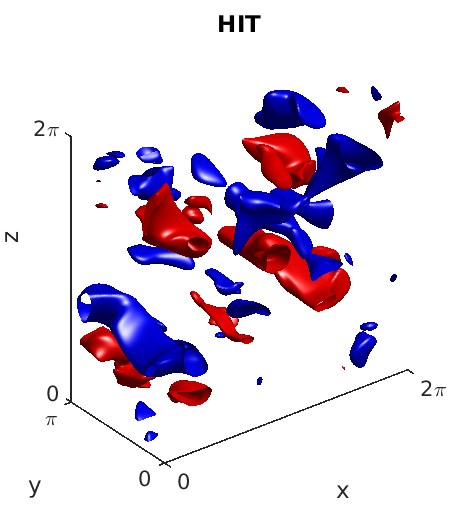
\includegraphics{prob1_2_HIT.pdf}
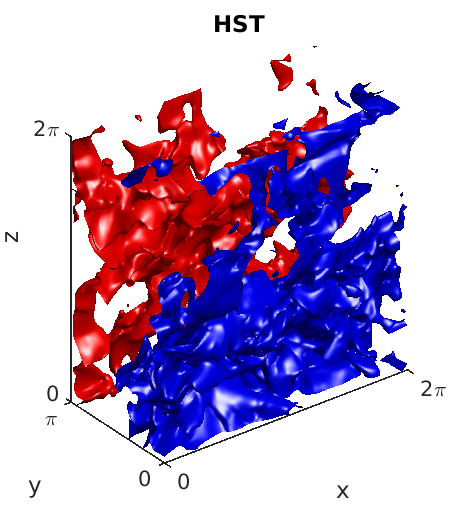
\includegraphics{prob1_2_HST.pdf}
\vspace{6pt}
\caption{Isosurfaces of $u$-velocity at half-max in red ({\color{red}$\blacksquare$}) and half-min in blue ({\color{blue}$\blacksquare$}) for HIT and HST.}
\label{fig:prob_1_2_isosurfaces}
\end{figure}

\subsection{}

\figref{fig:prob_1_3_slices} shows velocity fields $u$, $v$, and $w$ in all three slice planes located at $k = \{1, 128, 256\}$ for both the isotropic (HIT) and shear (HST) cases.

The isotropic (HIT) case has a much lower mean velocity and perhaps a larger viscous length scale, as velocity gradients are much smaller in magnitude compared to the shear (HST) case. This particular view of the HIT data, like the isosurface plots, shows a preferential axial direction of turbulent structures in the $j$-direction. As discussed previously, this could very well be transient.

Flow in the shear (HST) case is driven by opposing motion of the $y=0$ and $y=\pi$ bounding planes in the $i$-direction, and this manifests as a large velocity gradient of $u$ in all $xy$-slice planes. The velocities $v$ and $w$ are qualitatively similar, in that their distributions of velocities are similar. The only difference is that the structures in the $w$-field appear more elongated in the $i$-direction than those in the $v$-field at this instance in time.

Within each case, the velocity components at slice planes $k=1$ and $k=256$ are identical. This implies use of periodic boundary conditions, at least on the $z$-normal domain boundaries. Periodic boundaries are likely used on all bounding planes for HIT, and on the $z$- and $x$-normal bounding planes for HST. (We will see in a later part that the \emph{fluctuation} velocities are in fact periodic on all bounding faces for both HIT and HST.)

\begin{figure}[h!]
\centering
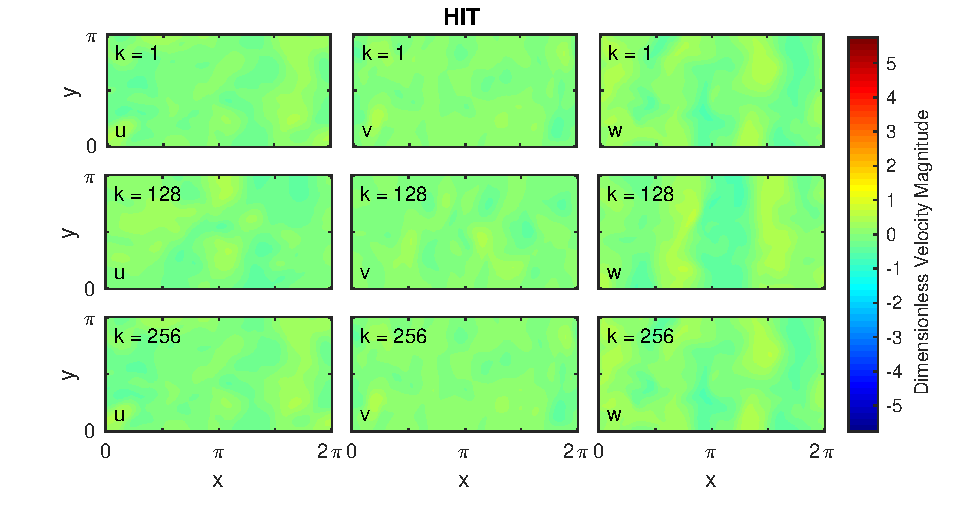
\includegraphics[trim=0.5cm 0cm 0cm 0cm]{prob1_3_HIT.pdf}
\\
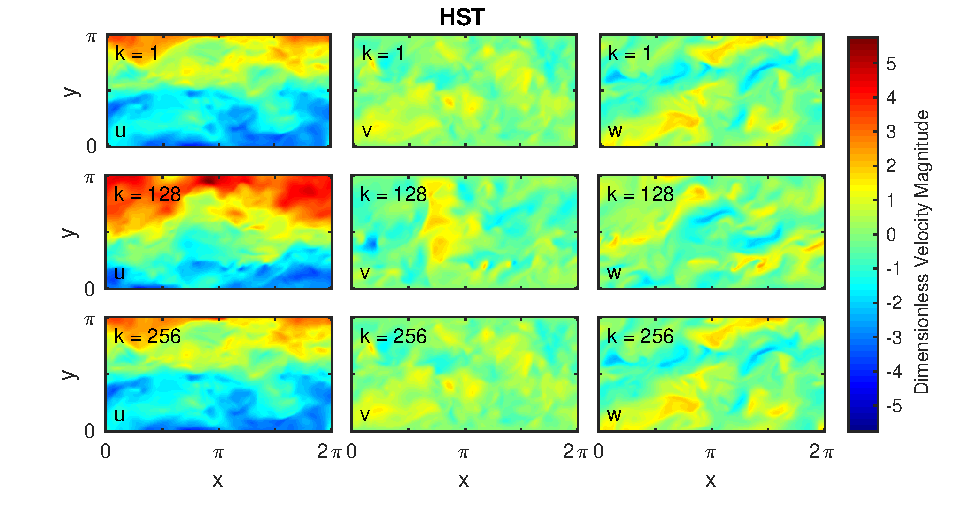
\includegraphics[trim=0.5cm 0cm 0cm 0cm]{prob1_3_HST.pdf}
\\[6pt]
\caption{Cartesian velocity components $u_i$ in three slice planes for the isotropic (HIT) and shear (HST) cases. Note that color scales are not identical between cases.}
\label{fig:prob_1_3_slices}
\end{figure}

\subsection{}

From the previous problems, we conclude that the homogeneous spatial directions for each case are: HIT ($i$, $j$, and $k$), and HST ($j$ and $k$). We expect the flow statistics to be invariant along these directions.

\subsection{}

We now calculate the $xz$-averages of all three velocity components for each turbulence case. That is, taking $u_i = \{ u, v, w \}$, we calculate
\begin{equation}
\expectation{u_i}_{xz}(y)
=
\frac{1}{XZ}
\int_{z_\text{min}}^{z_\text{max}}
\int_{x_\text{min}}^{x_\text{max}}
u_i(x,y,z) dx dz
.
\end{equation}
We wish to apply the definition to our discrete dataset. In discrete form, the integral becomes
\begin{equation}
\expectation{u_i}_{xz}(y)
\rightarrow
\frac{1}{N_x N_z}
\sum_{k=1}^{N_z}
\sum_{i=1}^{N_x}
u_i(i,j,k)
.
\end{equation}

Carrying out this calculation, we obtain the results shown in \figref{fig:prob_1_5_xzaverages}. The isotropic (HIT) case has near-zero $xz$-average velocity in all Cartesian directions for all $y$, though some minor fluctuations are observed in the $u$- and $w$-velocities. The shear (HST) case averages show $u$ varying linearly from $-3$ to $3$ as a function of $y$, whereas the other two components have zero average velocity, independent of $y$. Both observations confirm our expectations from the previous problem regarding homogeneous directions.

\begin{figure}[t]
\centering
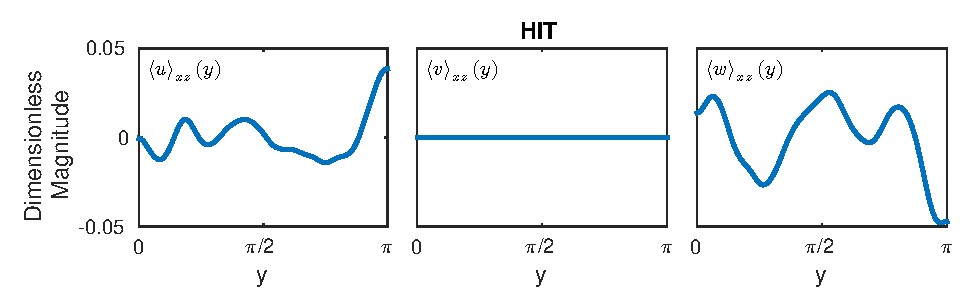
\includegraphics{prob1_5_HIT.pdf}
\\
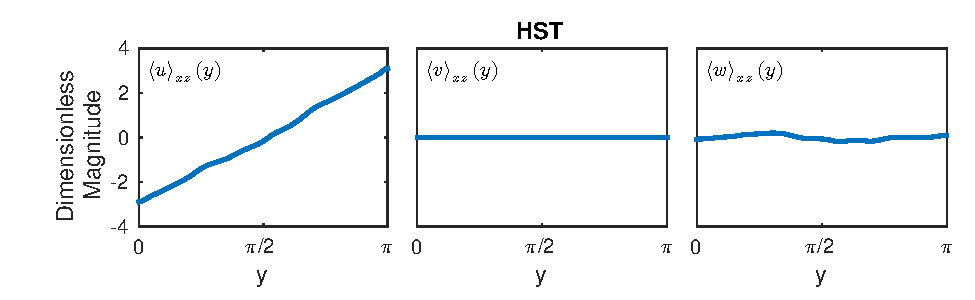
\includegraphics{prob1_5_HST.pdf}
\\[6pt]
\caption{Velocity $xz$-averages as a function of $y$-position for the isotropic (HIT) and shear (HST) turbulence cases. Note the disparate scaling between cases.}
\label{fig:prob_1_5_xzaverages}
\end{figure}

\subsection{}

We now subtract the $xz$-average velocities from the slice plane velocity components of Problem 1.3. The results of this calculation for the shear (HST) case,
\begin{equation}
u_i' = u(x,y,z) - \expectation{u_i}_{xz}(y)
,
\end{equation}
are shown in \figref{fig:prob_1_6_slices}. Comparing this to \figref{fig:prob_1_3_slices}, we see that $u_i$ and $u_i'$ are nearly identical for all but $u$. This is to be expected, since $\texpectation{u_i}_{xz}(y) \approx 0$ for all but $u$. In this unique case, we see periodic boundary conditions again emerge between the $y=0$ and $y=\pi$ bounding planes with respect to velocity \emph{fluctuation} rather than velocity itself. We also see that $\texpectation{u'}=0.63$ is positive in the midplane $k=128$, but that $\texpectation{u'}=-0.50$ is negative at the bounding planes, though this disparity could very well be transient.

\begin{figure}[h!]
\centering
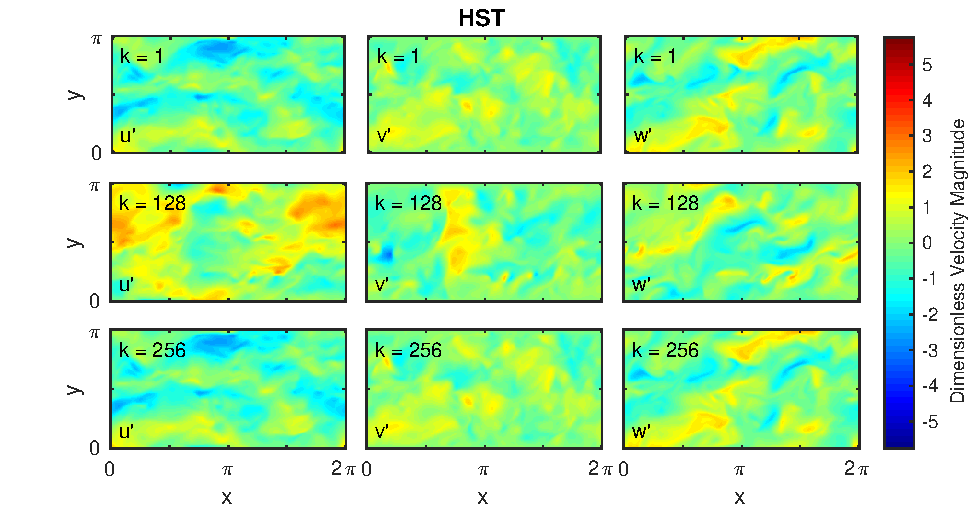
\includegraphics[trim=1cm 0cm 0cm 0cm]{prob1_6_HST.pdf}
\\[6pt]
\caption{Cartesian velocity fluctuation components $u_i' = u_i - \texpectation{u_i}_{xz}(y)$ in three slice planes for the shear (HST) case. Compare to \figref{fig:prob_1_3_slices}, which uses the same colorbar scale.}
\label{fig:prob_1_6_slices}
\end{figure}

\begin{figure}[h!]
\centering
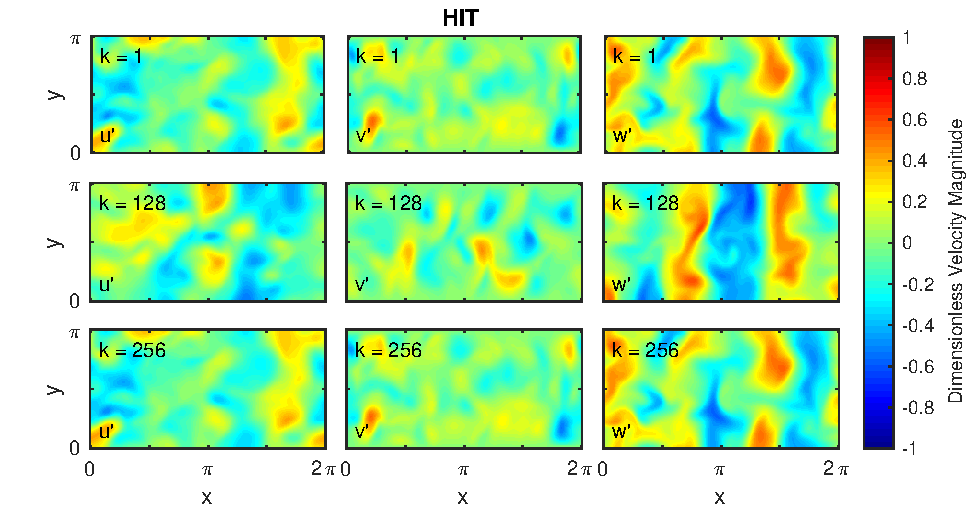
\includegraphics[trim=0.5cm 0cm 0cm 0cm]{prob1_7_HIT.pdf}
\\[6pt]
\caption{Cartesian velocity fluctuation components $u_i' = u_i - \texpectation{u_i}_{xyz}$ in three slice planes for the isotropic (HIT) case. Compare to \figref{fig:prob_1_3_slices}, which uses the same colorbar scale.}
\label{fig:prob_1_7_slices}
\end{figure}

\subsection{}

Next, we subtract the $xyz$-average velocities from the slice plane velocity components of Problem 1.3. The results of this calculation for the isotropic (HIT) case,
\begin{equation}
u_i' = u(x,y,z) - \expectation{u_i}_{xyz}
,
\end{equation}
are shown in \figref{fig:prob_1_7_slices}. Comparing this to \figref{fig:prob_1_3_slices}, we see that $u_i$ and $u_i'$ are nearly identical. This is expected since $\texpectation{u_i}_{xyz}$ is negligible compared to the average velocity magnitude of the isotrpic case.

\subsection{}

Reynolds stresses play an important role in fluid transport equations, and we turn to them now. For the shear (HST) case, we calculate $\texpectation{u_i' u_j'}_{xz}(y)$ to account for the anisotropic $y$-direction. In \figref{fig:prob_1_8_reynolds_stresses}, this is compared to the single-valued Reynolds stresses $\texpectation{u_i' u_j'}_{xyz}$ of the isotropic (HIT) case, represented as horizontal lines for each combination of $i$ and $j$. Some Reynolds stresses are redundant due to the commutative property of multiplication, and thus only unique stresses are shown.

All isotropic (HIT) Reynolds stresses are approximately zero, whereas non-zero values are almost entirely absent from the shear (HST) flow. Since Reynolds stresses act as production terms in the Reynolds-decomposed vorticity transport equation, it is unsurprising that such stresses manifest in a shear flow. The greatest shear stresses are $\texpectation{u'u'}_{xy}$ in the HST flow, corresponding to velocity fluctuations in the direction of applied shear.

\begin{figure}[t]
\centering
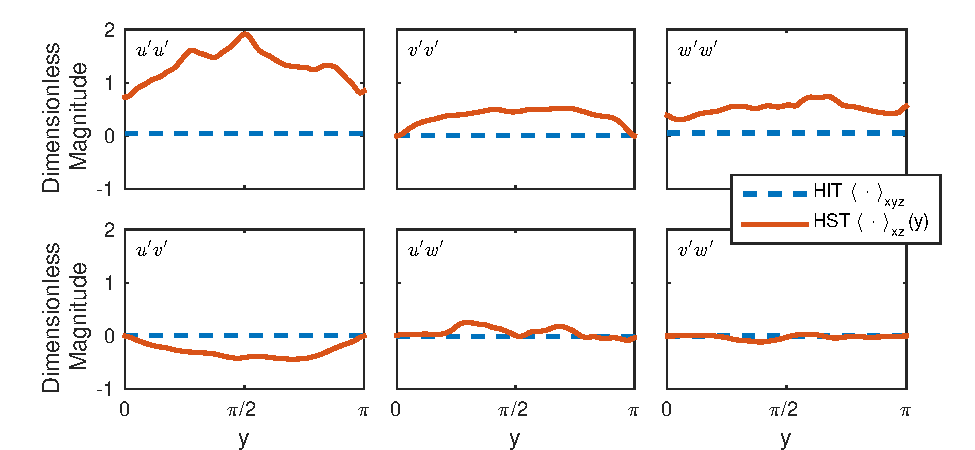
\includegraphics{prob1_8.pdf}
\\[6pt]
\caption{Independent Reynolds stresses for the isotropic (HIT) and shear (HST) cases. Note the HIT stresses have been averaged over the entire domain, whereas the HST stresses retain their $y$-dependence.}
\label{fig:prob_1_8_reynolds_stresses}
\end{figure}

\subsection{}

For the fluctuating velocity $u' = u - \texpectation{u}$, we now calculate the $n=\{2,3,4\}$ moments for the HIT and HST data using the appropriately defined averages $\expectation{u}$ in each case. Skewness and kurtosis values are obtained from these moments, and are plotted for each case in \figref{fig:prob_1_9_skew_kurtosis}.

Comparing the skewness and kurtosis of $u'$ for the two cases, it is apparent that neither matches a Gaussian distribution exactly. Both isotropic and shear turbulence exhibit higher skewness and lower kurtosis than a process governed by ideal Gaussian statistics. The presence of mean shear brings the skewness closer to that of Gaussian statistics compared to an isotropic flow. However, whereas the kurtosis of isotropic turbulence is within a few percent of the Gaussian value, mean shear significantly decreases the kurtosis.

\begin{figure}[t]
\centering
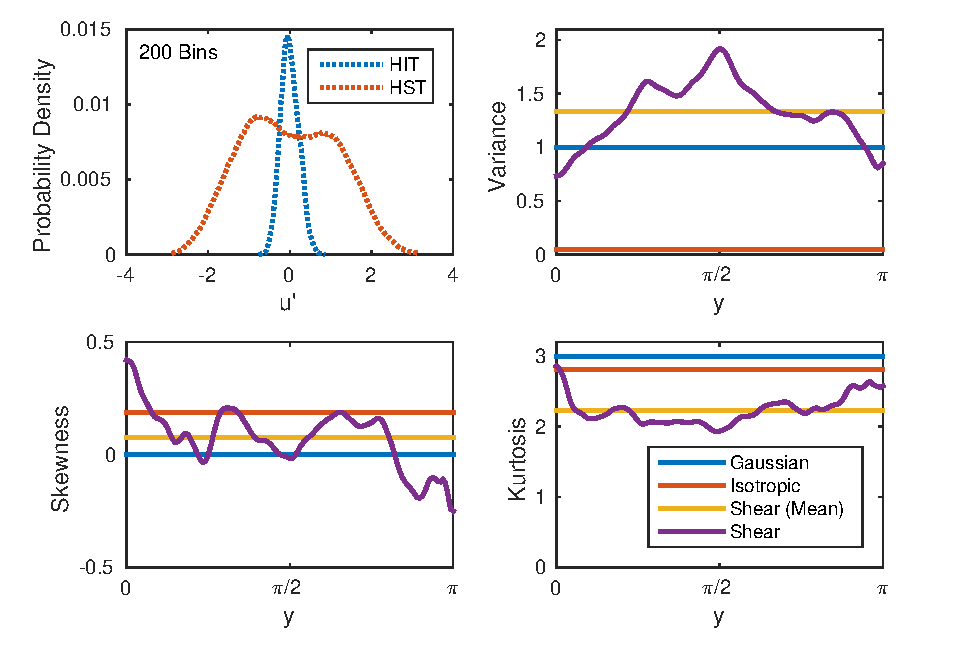
\includegraphics{prob1_9.pdf}
\vspace{-6pt}
\caption{Variance, skewness, and kurtosis of the isotropic (HIT) and shear (HST) fluctuation velocities. PDFs over the entire domain for both cases are included for qualitative reference, as are moments of an ideal Gaussian distribution. Shear moments are plotted as a function of $y$ as they are calculated using the PDF of $u'(y) = u - \expectation{u}_{xz}(y)$. Isotropic moments use $u' = u - \expectation{u}_{xyz}$, and are thus single-valued. For data processing, 1200 uniform bins over the interval $u' \in [-6,6]$ are used. However, the PDFs shown have been made independent of bin size, and reflect the continuous nature of the fluctuation velocities.}
\label{fig:prob_1_9_skew_kurtosis}
\end{figure}

\subsection{}

\figref{fig:prob_1_10_fluctuation_pdfs} shows the probability density functions of $u'$, $v'$, and $w'$ in the full volume for the isotropic (HIT) case, and in each of the three $xz$-planes at $j=\{32,64,96\}$ for the shear (HST) case. Gaussian distributions using the same mean and variance as each set of data are included for comparison.

From this plot, we can see that the PDFs of $u'$, $v'$, and $w'$ vary little between different values of $j$. Note that the difference in `roughness' is a direct consequence of sample size. The isotropic (HIT) PDFs appear similar to the shear (HST) PDFs, but the isotropic ones are better approximated by a Gaussian distribution, at least in the $x$- and $y$-directions. Both exhibit non-Gaussianity though: HIT has a far sharper peak at the center of the $v'$ distribution than a Gaussian would, and HST velocity fluctuations in the direction of applied shear ($u'$) are highly bimodal. The velocity magnitudes of the HST case, as has been previously discussed, have a wider range than the HIT case by about $6\times$.

These plots confirm that turbulent statistics are highly non-Gaussian, even in the isotropic case. The presence of mean shear increases the departure from Gaussian statistics, as evinced by the bimodal nature of the $u'$ PDFs. This \emph{suggests a disruption of the energy cascade} in flows with mean shear. That is, the preferential distribution of fluctuation velocities about two concentrations of equal non-zero magnitude suggests that they are ``bunching up'' there, and have a harder time transfering kinetic energy to smaller length-time scales.

\begin{figure}[t]
\centering
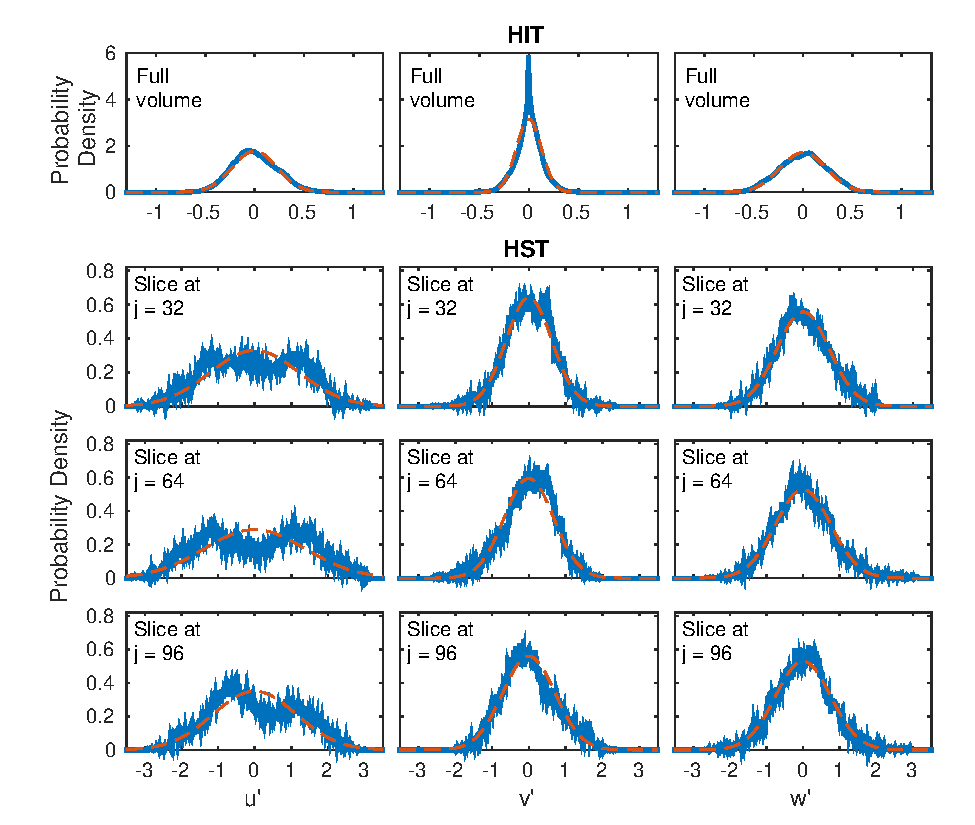
\includegraphics{prob1_10.pdf}
\\[6pt]
\caption{PDFs of fluctuation velocities (\legendline{blue,solid}), and corresponding Gaussian distributions (\legendline{orange,dashed}) with identical first and second moments for comparison. HIT statistics are calculated over the full domain, whereas HST statistics are shown in three different slice planes at $j = \{32,64,96\}$.}
\label{fig:prob_1_10_fluctuation_pdfs}
\end{figure}

\section{Analysis of Velocity Gradients in HIT}

\subsection{}

The volume average of the velocity gradient tensor is
\[
\expectation{A_{ij}}_{xyz} =
\begin{bmatrix*}[r]
 1.2382\e{-02} &  2.7474\e{-08} &  7.3195\e{-06} \\
-3.1956\e{-11} &  5.1524\e{-06} &  1.0050\e{-06} \\
-1.9175\e{-02} & -1.0693\e{-05} & -1.4207\e{-08}
\end{bmatrix*}
\]

\subsection{}

\subsection{}

\subsection{}

\subsection{}

\subsection{}

\subsection{}

\subsection{}

\subsection{}

\section{Advanced Topics}

\subsection{}

\subsection{}

\section{Extra Credit: The Biot-Savart Integral}

\section*{Appendex: \textsc{Matlab} Code}

%%
%% DOCUMENT END
%%
\end{document}












